\section{Προσαρμοσμένη Μάθηση}
\subsection{Μαθηματικός Ορισμός Μοντέλου Μάθησης}
Το \textlatin{ChronoQuest} θα έχει ένα σύστημα προσαρμοσμένης μάθησης. Η αρμοδιότητά του θα είναι η πιθανοτική αξιολόγηση με βάση τέσσερις παραμέτρους \cite{bkt_wiki}:
\begin{itemize}
    \item \textbf{$p_{init}(s)$}: Η πιθανότητα ο χρήστης να έχει γνώση πάνω σε κάποιο θέμα/ενότητα \textbf{$s$}.
    \item \textbf{$p_{learn}(s)$}: Η πιθανότητα ο χρήστης να μάθει το θέμα $s$ μετά από προσπάθεια
    \item \textbf{$p_{slip}(s)$}: Η πιθανότητα ο χρήστης να κάνει λάθος παρόλο τη γνώση του στο θέμα $s$
    \item \textbf{$p_{guess}(s)$}: Η πιθανότητα ο χρήστης να απαντήσει σωστά παρόλο τη έλλειψη γνώσης του στο συγκεκριμένο θέμα $s$
\end{itemize}

Οι παραπάνω παράμετροι είναι μέρος του αλγόριθμου γνωστού ως \textlatin{\textbf{Bayesian Knowledge Tracing (BKT)}}. Αυτός ο αλγόριθμος, με τη χρήση των τεσσάρων παραμέτρων, μας δίνει μια \textbf{πιθανότητα επιδεξιότητας} ενός χρήστη $u$ για ενα συγκεκριμένη θέμα $s$. Οι παρακάτω εξισώσεις μπορούν να εφαρμοστούν για την ενημέρωση του μοντέλου όταν αλληλεπιδρά ο χρήστης $u$:

(1) Αρχικοποίηση:
$$p(X_1, s, u) = p_{init}$$

(2) Υπό συνθήκη πιθανότητα όταν ο χρήστης απαντάει σωστά:
$$p(X_t\ |\ obs = correct, s, u) = \frac{p(X_t, s, u) \cdot (1 - p_{slip}(s))}{p(X_t,s,u) \cdot (1 - p_{slip}(s)) + (1 - p(X_t, s, u)) \cdot p_{guess}(s) }$$

(3) Υπό συνθήκη πιθανότητα όταν ο χρήστης απαντάει λάθος:
$$p (X_t\ |\ obs = wrong, s, u) = \frac{p(X_t, s, u) \cdot p_{slip}(s)}{p(X_t,s,u) \cdot p_{slip}(s) + (1 - p(X_t, s, u)) \cdot (1 - p_{guess}(s)) }$$

(4) Ενημέρωση της πιθανότητας επιδεξιότητας:
$$p(X_{t+1}, s, u) = p(X_t\ |\ obs, s, u) + (1 - p(X_t\ |\ obs, s, u)) \cdot p_{learn}(s)$$

(5) Πιθανότητα ο χρήστης να κατέχει την έννοια σε επόμενη αλληλεπίδραση:
$$p(C_{t+1}, s, u) = p(X_{t+1}, s, u) \cdot (1 - p_{slip}(s)) + (1 - p(X_{t+1}, s, u)) \cdot p_{guess}(s)$$

Το σύστημα προσαρμοσμένης μάθησης θα παίρνει αποφάσεις για ένα χρήστη με βάση την εξίσωση (5).

\subsection{Χρήση εντός του \textlatin{ChronoQuest}}

Το σύστημα \textlatin{BKT} που ορίστηκε παραπάνω, θα χρησιμοποιηθεί για την πρόβλεψη και την καταγραφή της απόδοσης του χρήστη στα διάφορα θέματα.

Ένα θέμα μπορεί να είναι η γεωγραφία του τόπου, ή η ιστορία του. Έτσι, η απόδοση του χρήστη θα αξιολογείται με βάσει αυτά τα θέματα. 

\subsection{Αλγόριθμος Υπολογισμού Απόδοσης}
Αν αποθηκεύσουμε κάθε πιθανότητα επιδεξιότητας που καταγράφεται του μοντέλου \textlatin{BKT} μπορούμε να κατασκευάσουμε ένα \textbf{ιστορικό επιδεξιότητας} του χρήστη για ένα θέμα.

\begin{figure}[H]
    \centering
    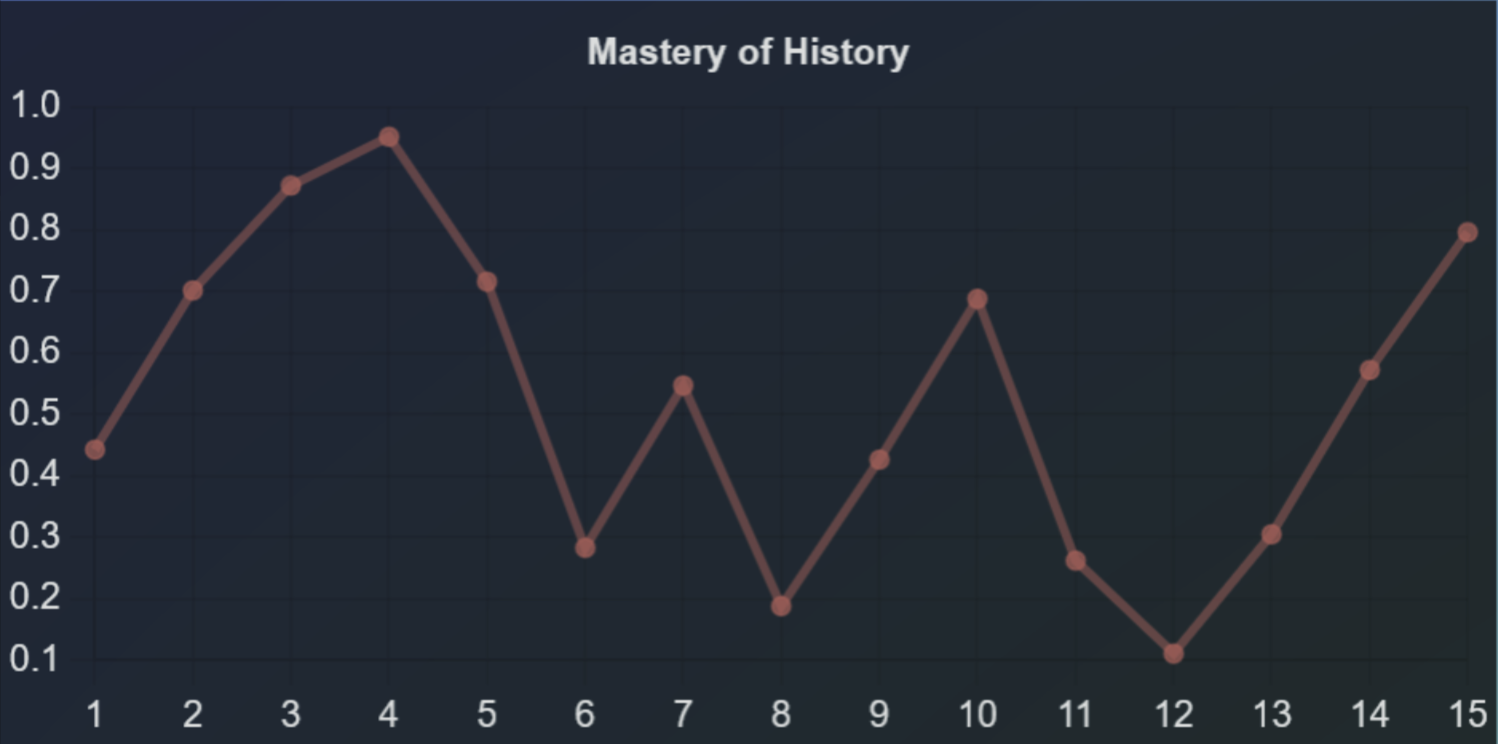
\includegraphics[width=0.5\linewidth]{img/MasteryGraph.png}
    \caption{Ιστορικό επιδεξιότητας}
\end{figure}

Ένας άνθρωπος μπορεί οπτικά μέσω του παραπάνω γραφήματος να βγάλει σωστά συμπεράσματα για την απόδοση του. Ας δούμε πως μπορούμε να "μαθηματικοποιήσουμε" την διαδικασία λήψης συμπερασμάτων.

Θα χρησιμοποιήσουμε 4 μετρικές για να αποκτήσουμε μια πολύ καλή εικόνα της απόδοσης του χρήστη:
\subsubsection{Ταχύτητα Μάθησης}
\subsubsection{Μοτίβα Απόκρισης}
\subsubsection{Αποδοτικότητα}
\subsubsection{Πρόοδος Μάθησης}
